%\part*{Lezione 15/03/2021}

\paragraph{Le basi della BBN} Innanzitutto elenchiamo gli \vir{ingredienti} essenziali della teoria:
\begin{itemize}
    \item Un network di reazioni.
    \item Il numero di neutroni e protoni di partenza, che sarà determinato, come abbiamo accennato, dalla vita media del neutrone, misura sulla quale tuttora è presente una certa incertezza (fornitaci dal PDG\footnote{PDG = Particle Data Group.}).
    \item Il rapporto tra barioni e fotoni detto \textbf{\textit{entropy factor}} $\eta$\index{entropy factor@\textit{entropy factor} $\eta$}\footnote{È definito come rapporto tra la densità barionica e quella dei fotoni $n_b/n_\gamma$.}. Questo parametro ci dice se è favorita la ricombinazione ($\eta$ grande) o la fotodisintegrazione della materia.
    \item Il fattore $\eta$ è legato alla \textbf{\textit{barion density}}\index{barion density@\textit{barion density} $\rho_B$} secondo $\rho_B = 6.8\cdot\ord{-22}\unit{g cm}^{-3}\; \cdot \eta$. Spesso però al posto di questa si tende a lavorare con la \textbf{\textit{barion fraction of critical mass density}}\index{barion fraction of critical mass density@\textit{barion fraction of critical mass density} $\Omega_B h^2$}, definita\footnote{Dove $h$ è un parametro adimensionale per la costante di Hubble, definito come $h=H_0/100 [\mbox{km}/\mbox{s Mpc}]$.} come $\Omega_B h^2= 3.6 \cdot\ord{7}\;\cdot \eta$.
\end{itemize}
Come \vir{output} da questi avremo le abbondanze degli elementi primordiali (ovvero H, He e metalli leggeri). Passiamo allora alla trattazione di questi \vir{input}.

\section{Network di reazioni}
In Figura \ref{0315_net} riportiamo le reazioni coinvolte nella nucleosintesi primordiale; nel seguito con i numeri puntati tra parentesi (per esempio (1.), (2.)) faremo riferimento alle reazione riportate in questa figura.
\begin{figure}[h]
    \centering
    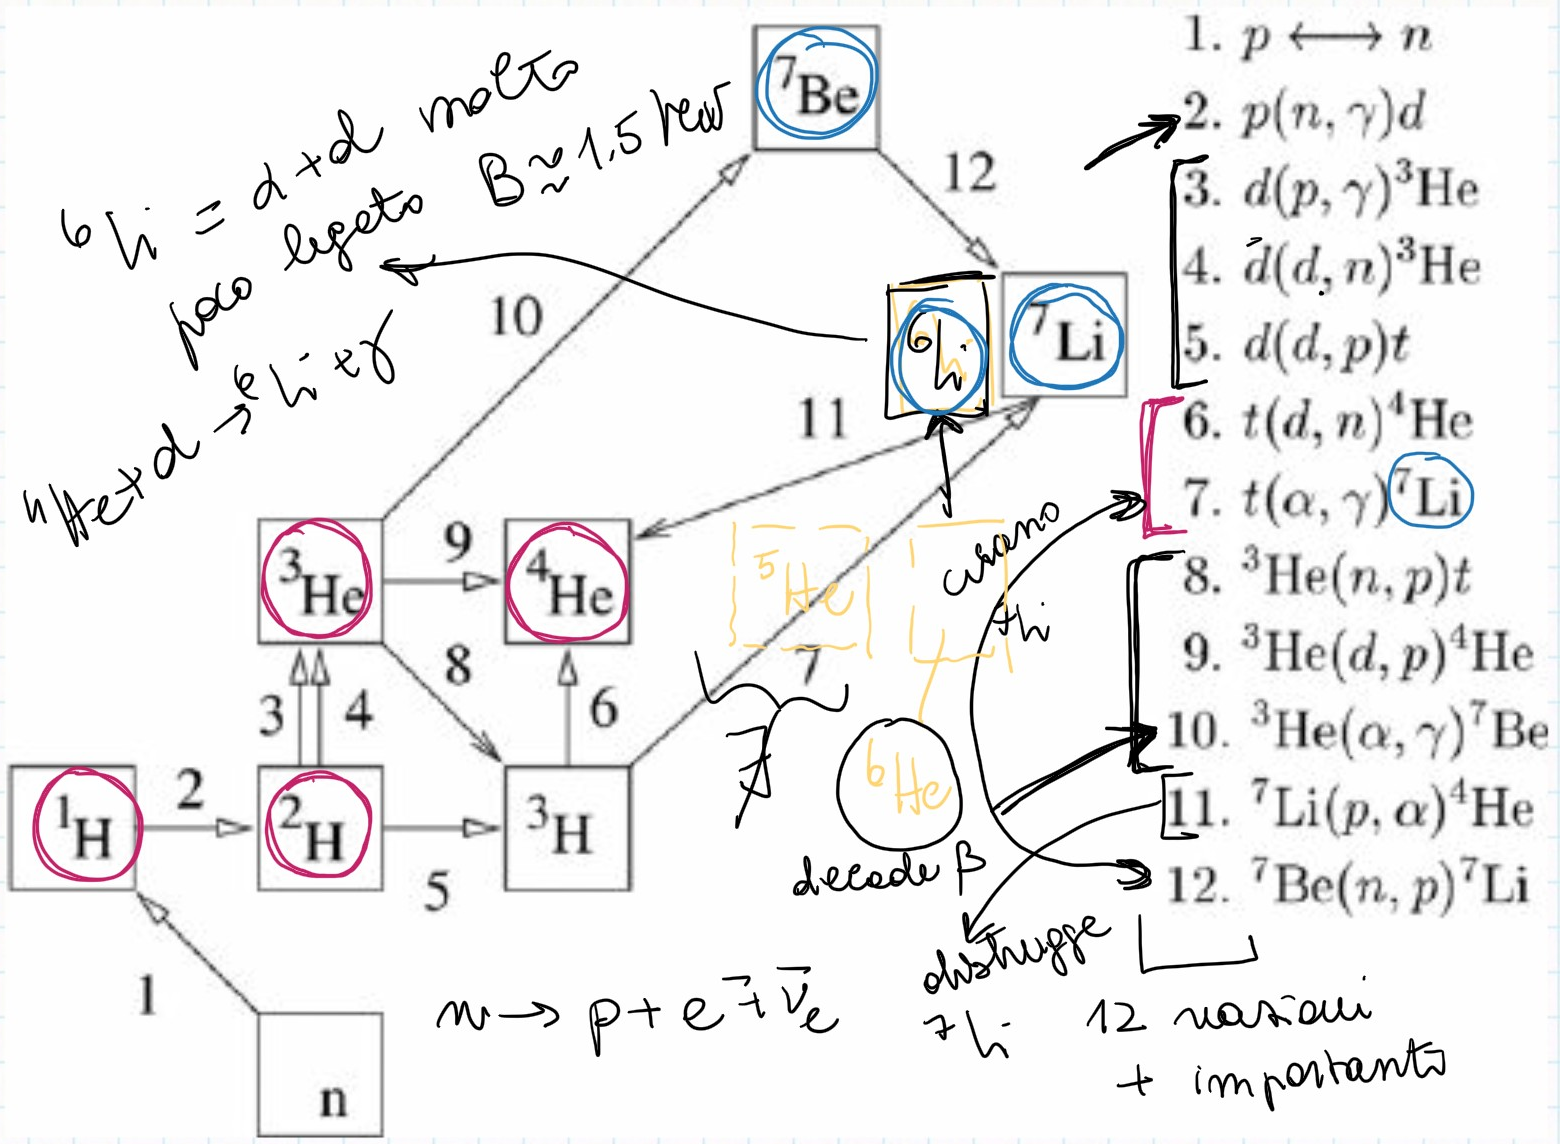
\includegraphics[scale=0.25]{Immagini/0315_network.png}
    \caption{Sono riportate le 12 reazioni più importanti. Gli elementi segnati in rosa sono i primordiali più abbondanti.}
    \label{0315_net}
\end{figure}

\paragraph{Criteri qualitativi di reazione} Prima di procedere ricordiamo alcune regole qualitative per capire quale tra i vari rami di una reazione è favorito rispetto agli altri:
\begin{itemize}
    \item[I.] $\sigma_\text{forte}\gg\sigma_\text{EM}\gg\sigma_\text{debole}$. Per riconoscere a quale tipo di interazione appartiene la reazione è sufficiente osservare i prodotti: se compaiono neutrini l'interazione è debole, se invece il numero di protoni e neutroni è conservato abbiamo interazione forte e se si ha anche produzione di un fotone allora si ha interazione elettromagnetica.
    \item[II.] L'abbondanza dei reagenti è discriminante.
    \item[III.] La barriera Coulombiana da superare per avere la reazione è un fattore che influisce fortemente sulla probabilità di reazione.
\end{itemize}

\subsection{La nucleosintesi primordiale}\label{sec-nuc-prim}
La prima reazione che abbiamo è il decadimento del neutrone\footnote{Si tratta dell'unica reazione di interazione debole.} (1.); successivamente segue una cattura radiativa $p$-$n$ (2.) e a questo punto abbiamo 3 possibili reazioni di distruzione del deuterio: secondo il I criterio la (4.) e la (5.) dovrebbero contare maggiormente rispetto alla (3.), ma poiché l'abbondanza di $p$ è superiore a quella di $d$ le probabilità delle tre reazioni sono dello stesso ordine\footnote{Si capisce allora come mai non si ha $d(d,\gamma)\ce{^4He}$ (poca abbondanza e interazione EM).}. Queste reazioni non sono sufficienti a consumare tutto il deuterio, che potrà interagire con il trizio $t$ secondo la (6.); il trizio non è un elemento primordiale perché decade\footnote{A titolo informativo: $t \to \ce{^3He}+e^-+\bar{\nu}_e$.}, ma essendo un decadimento debole è molto probabile che interagisca nuovamente con $\alpha$ (7.) dando $\ce{^7Li}$\footnote{Vedremo che la presenza di questo $\ce{^7Li}$ sarà una questione delicata da trattare.}.
Per quanto riguarda $\ce{^3He}$, invece, questo è stabile e ha varie reazioni di distruzione\footnote{Esisterebbe anche $\ce{^3He}(n,\gamma)\ce{^4He}$, ma la (8.) (data l'abbondanza e la natura dell'interazione) è molto più importante.}, tra cui la più importante se ancora vi sono neutroni è la (8.), alla quale segue (nonostante la poca abbondanza di deuterio) la (9.) e quando si raggiunge un certo numero di $\ce{^3He}$ e $\alpha$ si ha anche la (10.); ora il berillio che si è formato da questo viene distrutto praticamente tutto in $\ce{^7Li}$ (12.).\\
Fermiamoci un attimo: come mai non troviamo reazioni per $\ce{^5He}$, $\ce{^6He}$ e $\ce{^6Li}$? Allora il $\ce{^5He}$ non è uno stato legato, ma $\ce{^6He}$ sì, tuttavia questo decade $\beta$ molto velocemente (è poco legato) in $\ce{^6Li}$. Quest'ultimo si ottiene anche da $\alpha + d$ con l'emissione di un fotone e il motivo per cui la sua abbondanza non è significativa è dovuto al fatto che è poco legato, per cui si rompe facilmente.\\
Abbiamo ancora un problema da risolvere, ovvero che la carta dei nuclei presenta un \textit{gap} per $A=8$: il $\ce{^8B}$ e il $\ce{^8Li}$ decadono $\beta$ e il $\ce{^8Be}$ decade $\alpha$. Dunque, la BBN si ferma qui\footnote{In realtà esistono reazioni per saltare da $A=5$ ad $A=7$, ma sono comunque trascurabili rispetto a tutti gli altri processi.} con $p$, $\ce{^2H}$, $\ce{^3He}$, $\ce{^4He}$, $\ce{^7Li}$ (poco) e $\ce{^7Be}$ (pochissimo).

\paragraph{Confronto con le osservazioni} A questo punto per studiare la BBN è necessario prendere i valori delle varie sezioni d'urto delle reazioni coinvolte e vederne l'evoluzione temporale, come mostrato in Figura \ref{0315_mfrac}, dove è riportata la \textit{mass fraction} dei principali elementi predetta dal modello\footnote{Una piccola nota sul berillio: non è facile da misurare, quindi spesso quello che si misura è il rapporto $d/\ce{H}$ o $\ce{^3He/H}$.}. Dunque, dalle misure di queste quantità è possibile stimare la bontà della teoria.

\begin{figure}[!h]
    \centering
    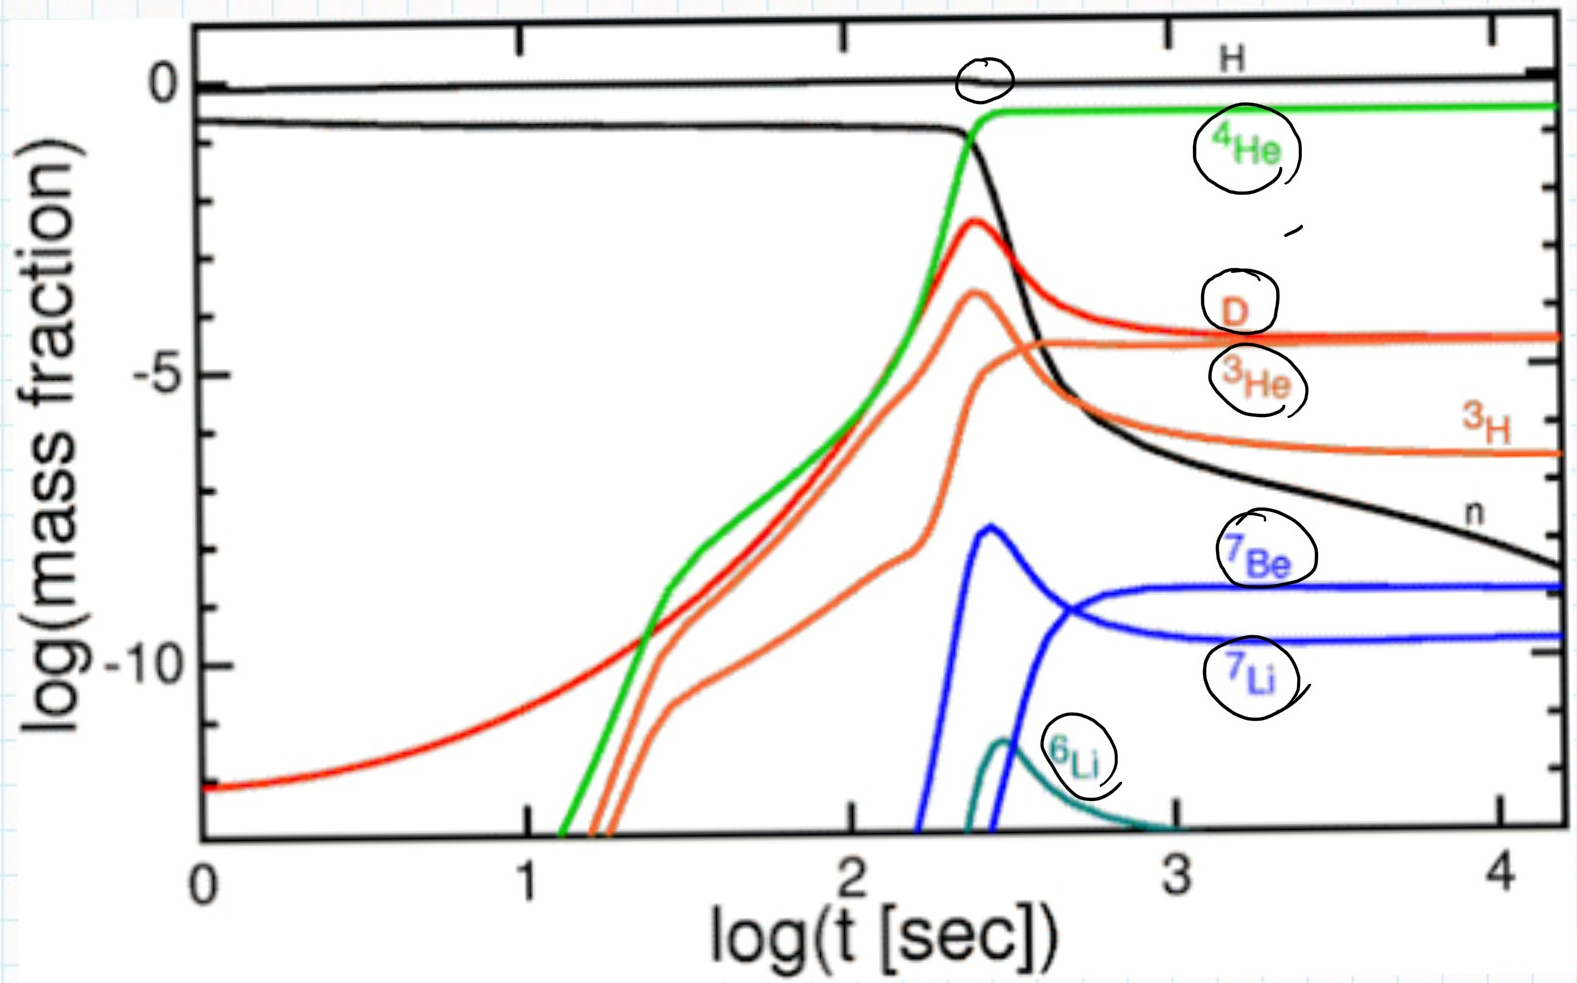
\includegraphics[scale=0.2]{Immagini/0315_massfraction.png}
    \caption{Andamento nel tempo della \textit{mass fraction}, ovvero dell'abbondanza di un elemento sull'abbondanza di $\ce{H}$. L'abbondanza di $\ce{H}$ ha un leggero scalino e quello segna l'inizio della BBN; si vede che $n$ decade; il $\ce{^3H}$ è indicato, ma decade; vi è un errore per l'andamento del $\ce{^6Li}$, dovrebbe essere più alto.}
    \label{0315_mfrac}
\end{figure}

\noindent Riportiamo allora le osservazioni in Figura \ref{0315_mfrac2}. Da queste misure è possibile stimare $\Omega_B h^2$ e alla fine degli anni '90 si ebbe la prima evidenza che la densità di materia dell'Universo fosse differente da quella attesa (a causa dell'assenza nel conto del contributo dovuto alla materia oscura). 

\begin{figure}[!h]
    \centering
    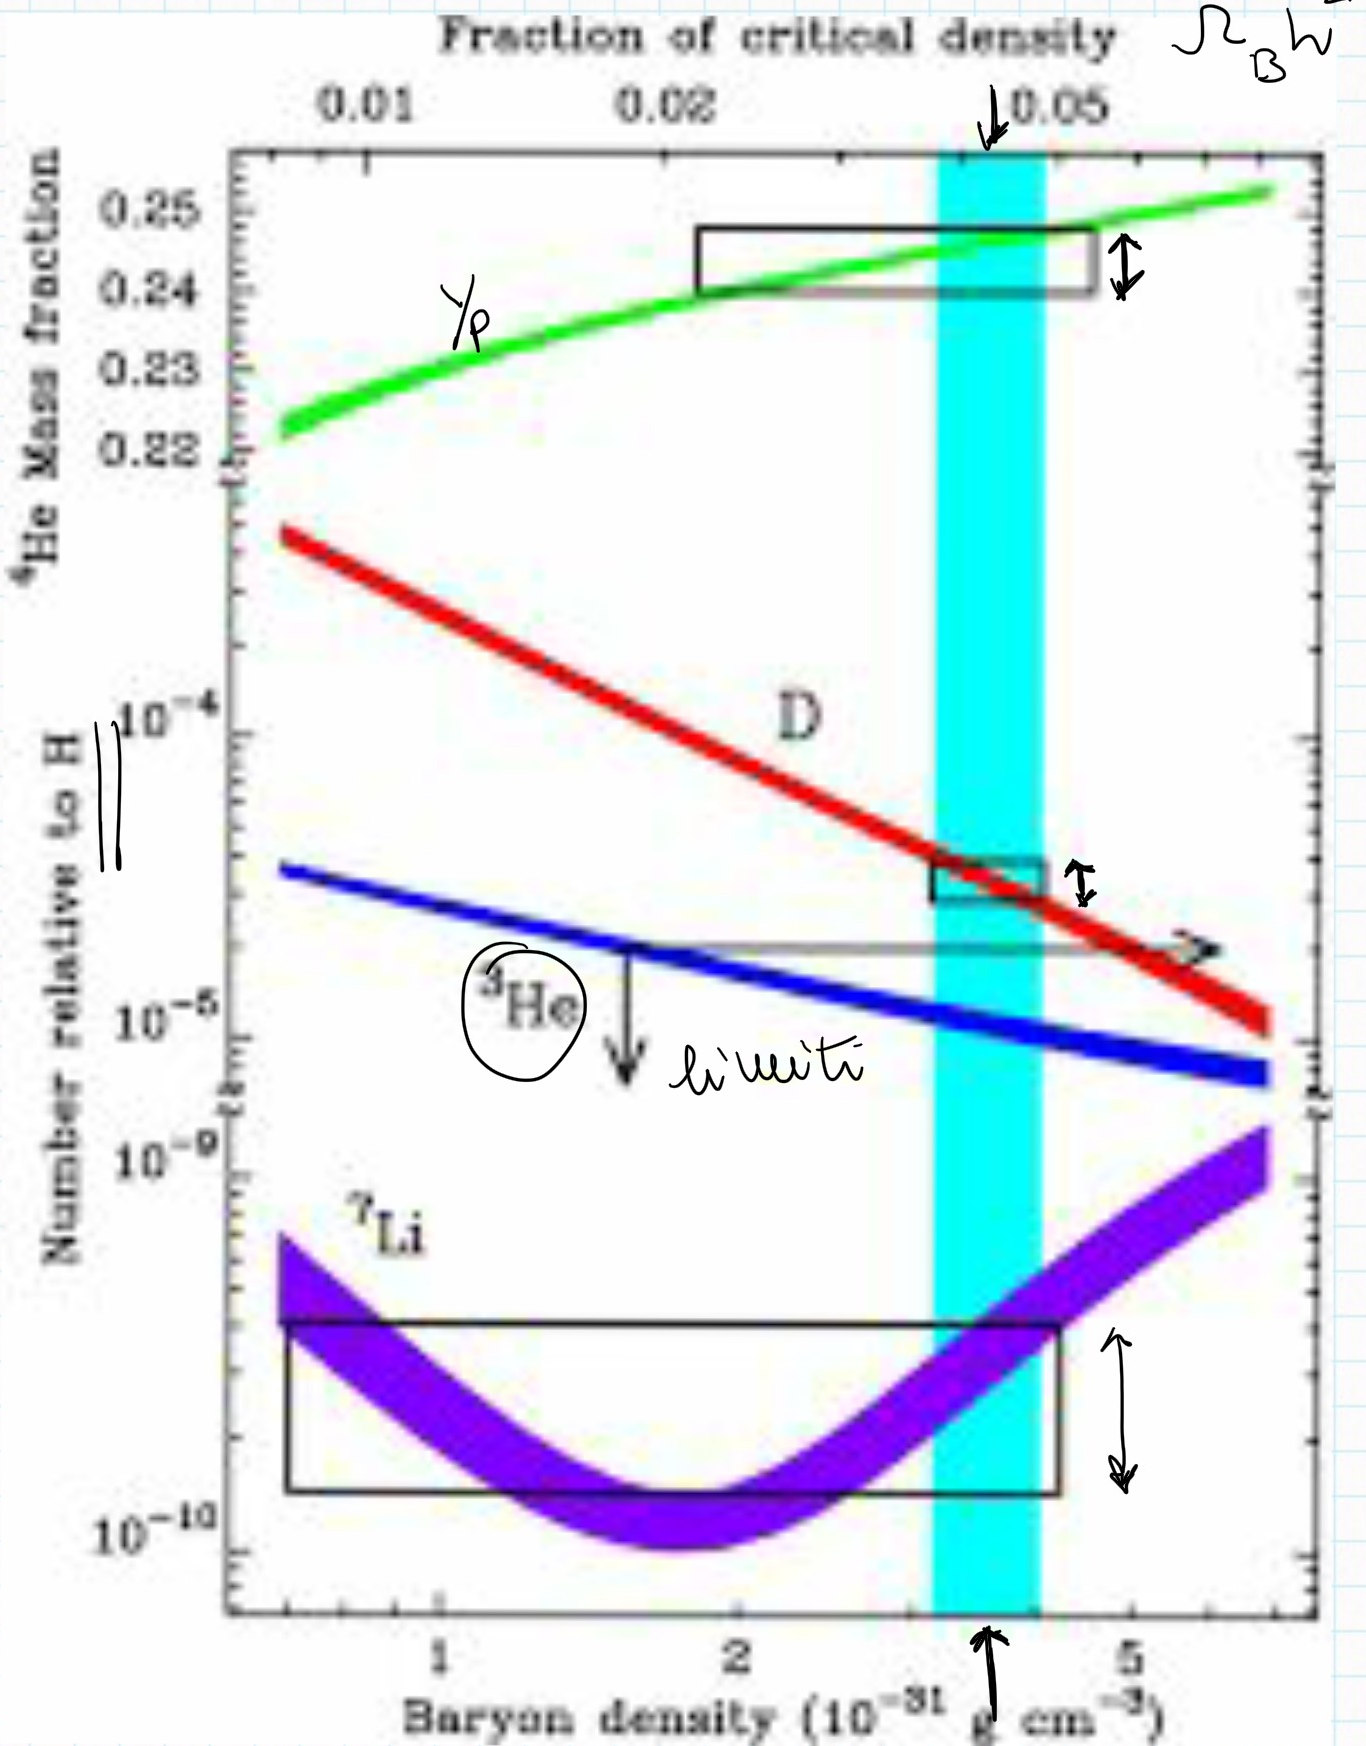
\includegraphics[scale=0.2]{Immagini/0315_massfraction2.png}
    \caption{Le bande degli andamenti sono dovute alle incertezze. Coi rettangoli si riportano le misure. Il range di interesse è indicato dalla striscia celeste. Per il trizio ci sono solo limiti superiori e inferiori.}
    \label{0315_mfrac2}
\end{figure}
\newpage
\paragraph{Misura delle abbondanze primordiali} Partiamo dalla misura per $\ce{^4He}$. I primi problemi sorgono dal fatto che le stelle ne hanno aumentato la concentrazione, dunque si fanno misure del rapporto $\ce{^4He}/\ce{H}$ in regioni in cui è avvenuta poca o quasi nulla evoluzione stellare, ovvero galassie \textit{metal-poor}. Riportiamo in Figura \ref{0315_Hefrac} un esempio. A oggi si ha un valore di circa $Y_p \sim 0.25$.

\begin{figure}[!h]
    \centering
    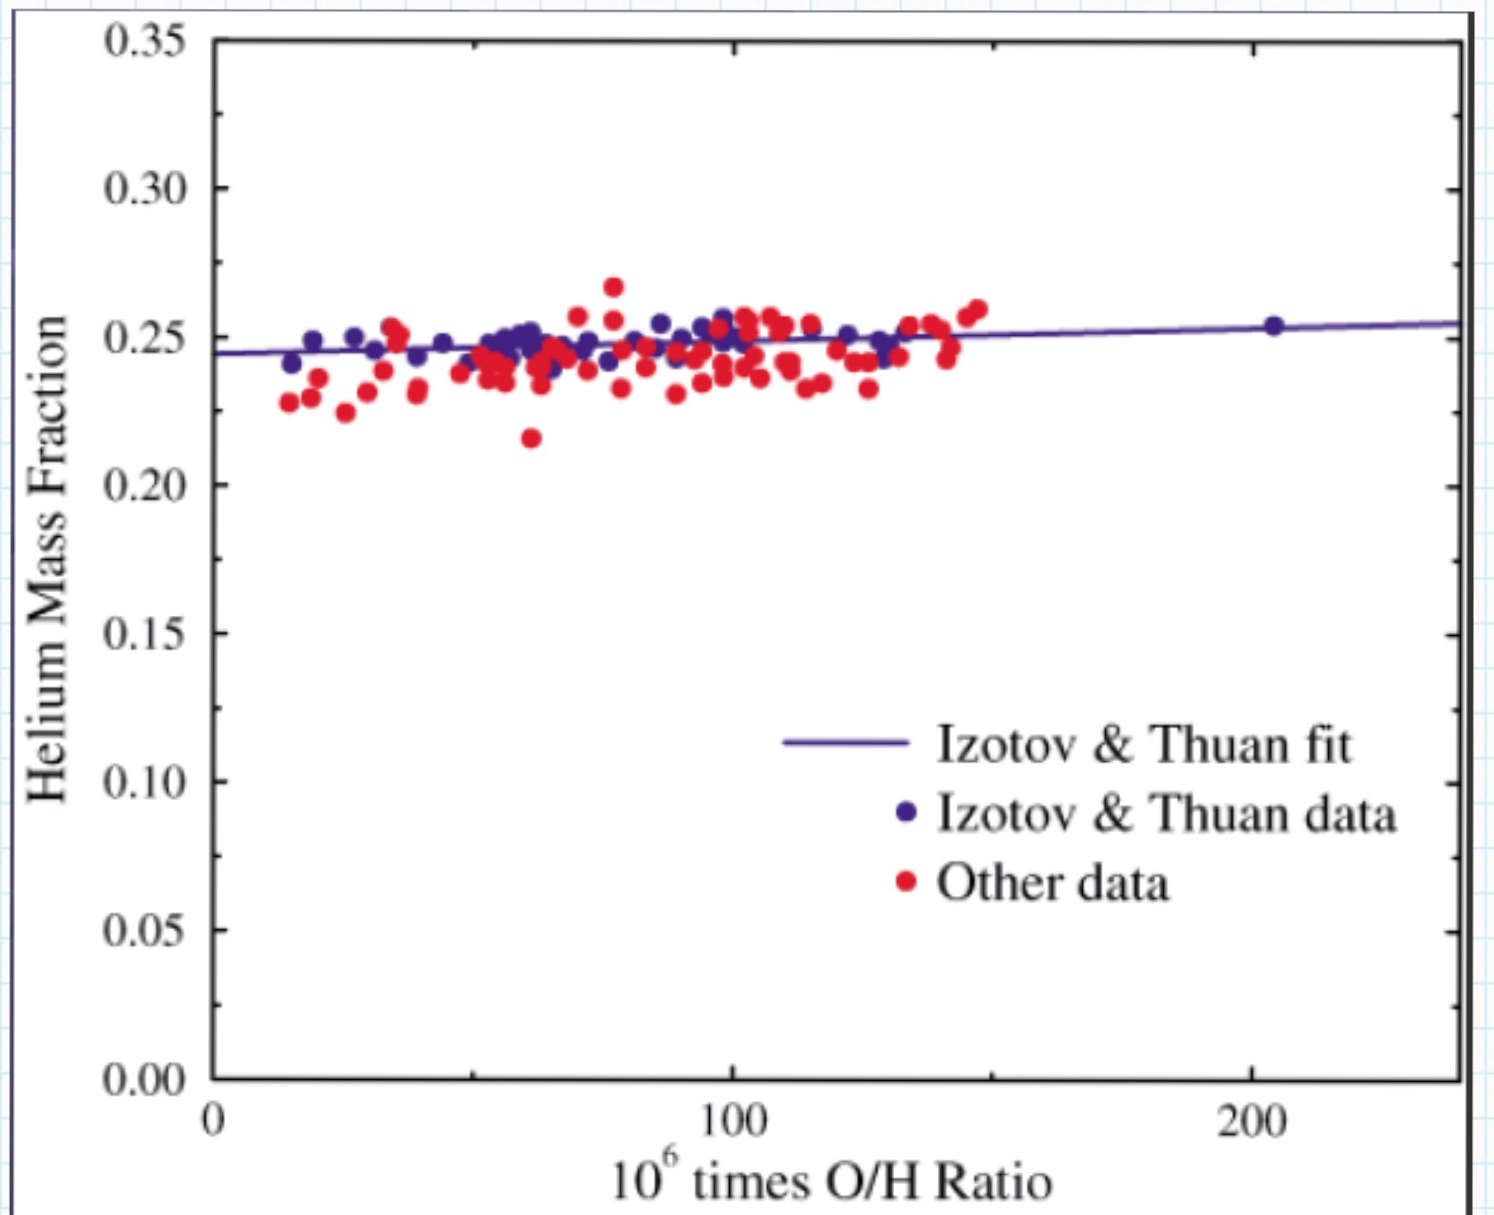
\includegraphics[scale=0.2]{Immagini/0315_heliummassfraction.png}
    \caption{Risultati sperimentali per stelle con metallicità differente.}
    \label{0315_Hefrac}
\end{figure}

\noindent La misura del deuterio è anche più problematica: esso infatti è \vir{fragile}, per cui vanno evitate le stelle e gli oggetti densi, anzi si fanno osservazioni nel mezzo interstellare.\\
Il 1973 il satellite Copernico riuscì a dare dei limiti (superiori e inferiori), ma non a raccogliere dei veri e propri dati. Successivamente, nel 1998, Tytler e Burles ebbero un'idea, ovvero quella di misurare $d/\ce{H}$ nelle \textit{hydrogen clouds} ad alto \textit{redshift}\index{redshift@\textit{redshift}} ($z>3$, oggetti molto vecchi): si osservano le linee di assorbimento della Ly$\alpha$\index{Lymann@Lymann $\alpha$} in \textit{quasi-stellar object}\index{quasi-stellar object@\textit{quasi-stellar object}} con metallicità $Z \sim \ord{-2}\div\ord{-3} Z\sol{}$ (per cui ci aspettiamo che l'abbondanza sia quella primordiale). A oggi il valore più accurato riporta $d/\ce{H} = (2.527 \pm 0.030)\cdot\ord{-5}$; questa accuratezza deriva dal fatto che l'abbondanza di deuterio è particolarmente sensibile alla densità di barioni.\\
Per quanto riguarda $\ce{^3He}$, anche questo è molto fragile e non dev'essere cercato nel mezzo interstellare, tuttavia la misura è complicata.\\
Il $\ce{^7Li}$, invece, viene ricercato nelle atmosfere stellari di stelle di popolazione II\index{popolazione II}, ovvero \textit{low-metallicity stars}\index{low-metallicity stars@\textit{low-metallicity stars}} (che si possono osservare nell'alone della nostra galassia). In Figura \ref{0315_LiH} riportiamo i dati sperimentali per il rapporto $\ce{^7Li}/\ce{H}$: notiamo dei dati (sulla destra) molto \vir{diffusi} che però non sono di interesse poiché si riferiscono a metallicità alte; per quanto riguarda gli altri dati (sulla sinistra) vi è tuttora ancora discussione riguardo il valore di $\ce{Fe}/\ce{H}$ oltre il quale fermarsi per il fit. Negli ultimi tempi queste misure sono diventate più accurate e hanno portato a un valore stimato di $\Omega_B h^2$ diverso da quello ottenuto dal $(\ce{^4He},d)$, dando vita a quello che oggi viene definito \textit{$\ce{Li}$-problem} (o \textit{puzzle}) della BBN\index{Li-problem@\textit{$\ce{Li}$-problem}}\index{Li-puzzle@\textit{$\ce{Li}$-puzzle}}.

\begin{figure}[!h]
    \centering
    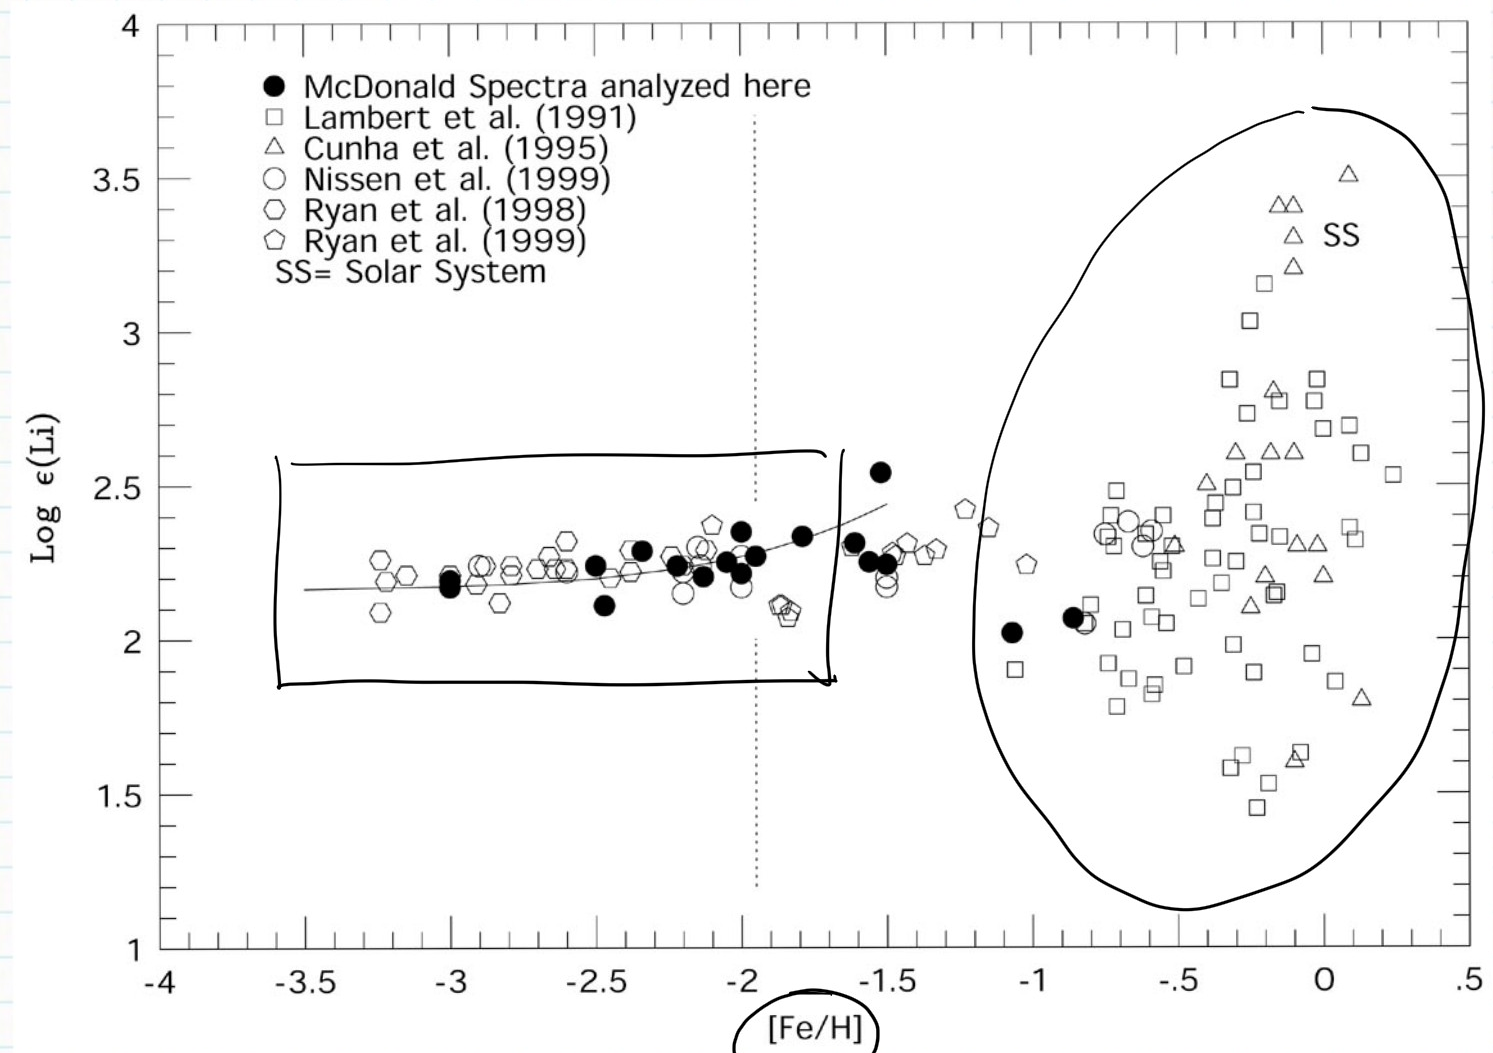
\includegraphics[scale=0.25]{Immagini/0315_LiH.png}
    \caption{\textit{Splite Plateau} per il $\ce{Li}$. Con $\varepsilon (\ce{Li})$ si indica la \textit{mass fraction} del litio.}
    \label{0315_LiH}
\end{figure}
\newpage
\section{La BBN e i neutrini}
Alla fine degli anni '90 la teoria della BBN era ormai supportata dall'accordo con evidenze sperimentali nell'abbondanza di 3 degli elementi più presenti nell'universo, %
% Compare negli appunti un "per = Omega_B"
acquisendo così un potere predittivo. Fu quindi impiegata per stimare il valore atteso per il numero di neutrini cosmici o per meglio dire la \textit{radiation density}\index{radiation density@\textit{radiation density} $N_\nu$} $N_\nu$ (l'osservabile che effettivamente si misura). All'interno del modello un aumento delle specie di neutrini comporterebbe un aumento nella densità di energia dell'universo, ovvero una crescita del rate di espansione e di conseguenza un anticipo del \textit{Freeze-out}\index{Freeze-out@\textit{Freeze-out}}: $H^2 \propto N_\nu T^4$, dunque se $N_\nu $ è maggiore allora $T$ è minore. Se riprendiamo l'esempio che avevamo fatto nel paragrafo \vir{\textbf{A grandi linee}} a pg. \pageref{a.grandi.linee} per il numero di neutroni al \textit{Freeze-out} si ha in questo caso:
$$N_n = N_0 e^{-t/\tau} = 220 e^{-100/886} \simeq 196$$
Abbiamo quindi un maggior numero di neutroni e questo comporta una densità di $\ce{^4He}$ più alta. Riportiamo in Figura \ref{0315_Hefrac2} l'andamento della \textit{mass fraction} per l'elio al variare della $N_\nu$.

\begin{figure}[!h]
    \centering
    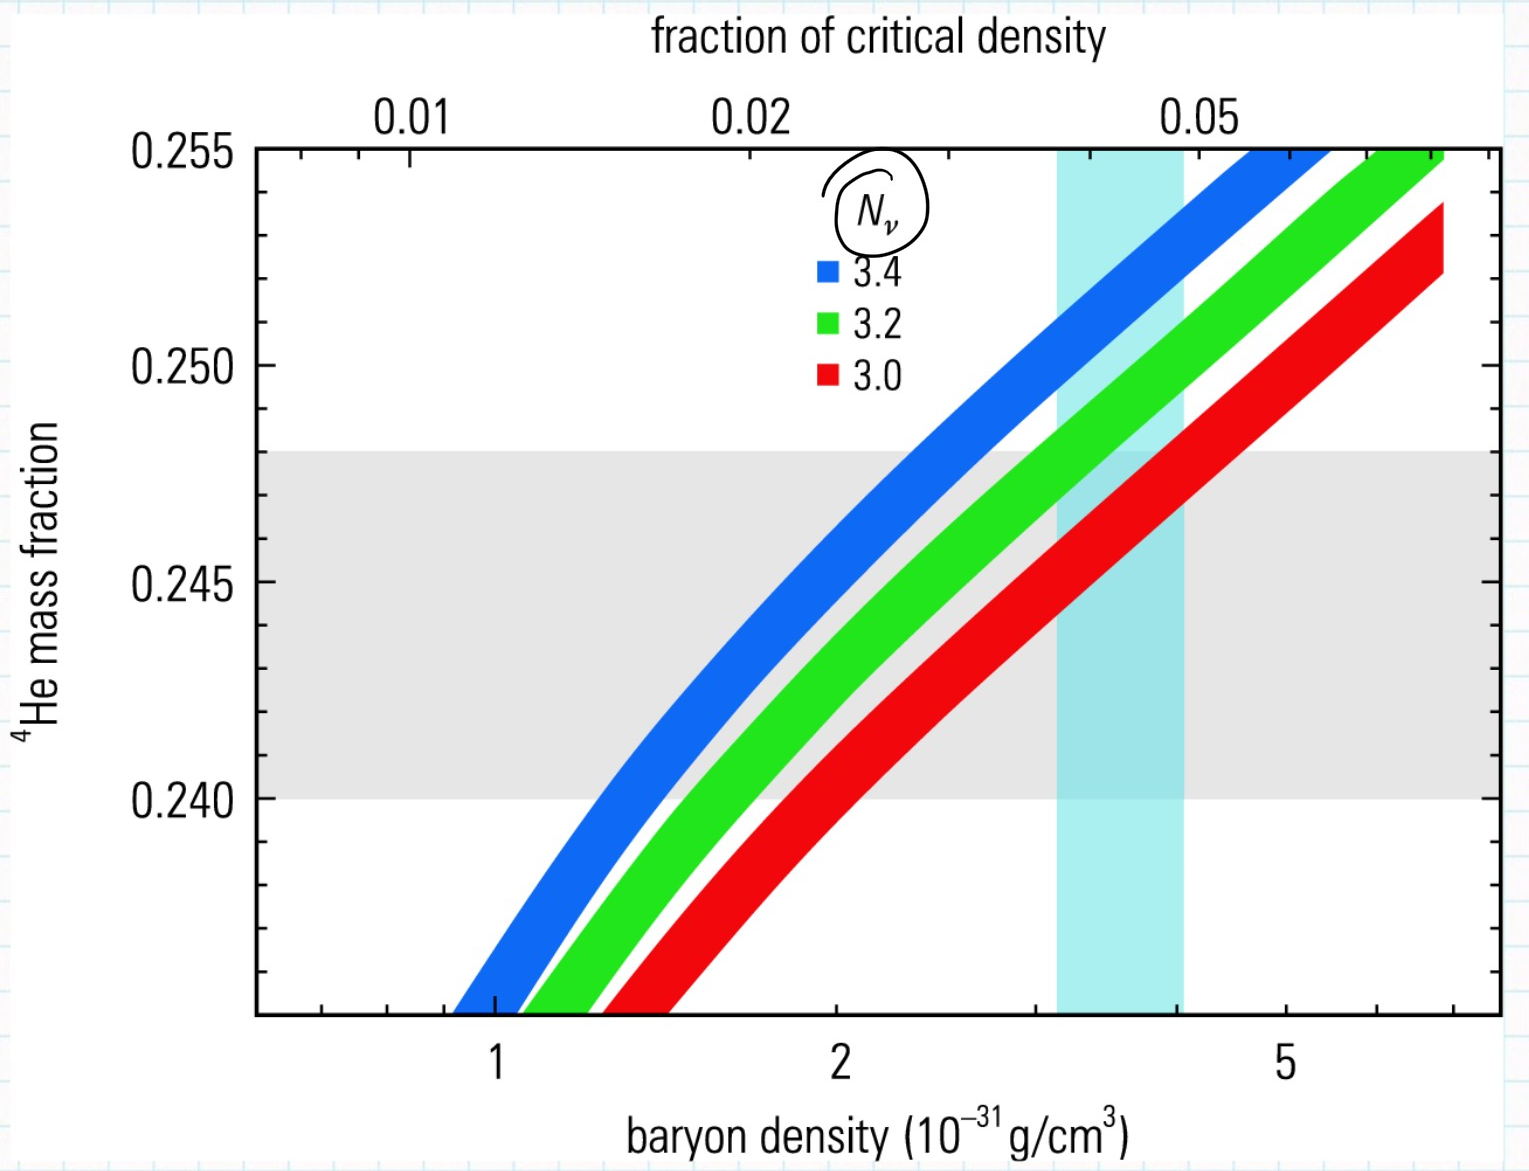
\includegraphics[scale=0.2]{Immagini/0315_heliummassfraction2.png}
    \caption{La banda grigia rappresenta i dati sperimentali. Data la densità dei barioni si evince che gli andamenti per $N_\nu = 3.4$ e $3.2$ vadano esclusi.}
    \label{0315_Hefrac2}
\end{figure}



\section{La BBN oggi}
La teoria della BBN oggi si basa sul modello cosmologico standard\index{modello cosmologico standard@modello cosmologico standard $\Lambda CDM$} $\Lambda CDM$\footnote{L'acronimo:%
\begin{itemize}
    \item[$\Lambda$] sta per la costante cosmologica\index{costante cosmologica@costante cosmologica $\Lambda$}.
    \item[$CDM$] sta per \textit{Cold Dark Matter}.
\end{itemize}
}.\\
Di recente $\Omega_B h^2$ è stato misurato dal CMB ed è quindi possibile fare delle stime sulle abbondanze: il $d/\ce{H}$, per esempio, che è particolarmente sensibile al valore di $\Omega_B$ e a $N_\nu$\footnote{Da qui in poi chiameremo $N_\nu$ con $N_{eff}$.} e per il quale abbiamo una serie di reazioni che lo creano e lo distruggono\footnote{Fino al 2020 l'ultima era la più incerta.}:
\begin{displaymath}
\begin{aligned}
n + p &\to d + \gamma & &\text{Creazione} \\
d + d &\to \ce{^3He} + n & \\
d + d &\to \ce{^3H}  + p &  &\text{Distruzione} \\
p + d &\to \ce{^3He} + \gamma & 
\end{aligned}
\end{displaymath}
Quello che si misura effettivamente è il \textbf{fattore astrofisico}\index{fattore astrofisico@fattore astrofisico $S(E)$}\footnote{Si veda la sezione \secrif{sec-SE} per la definizione} $S(E)$, che ha le dimensioni di una sezione d'urto per un'energia; si riportano i risultati sperimentali per l'ultima reazione di distruzione in Figura \ref{0315_astr}.

\begin{figure}[h]
    \centering
    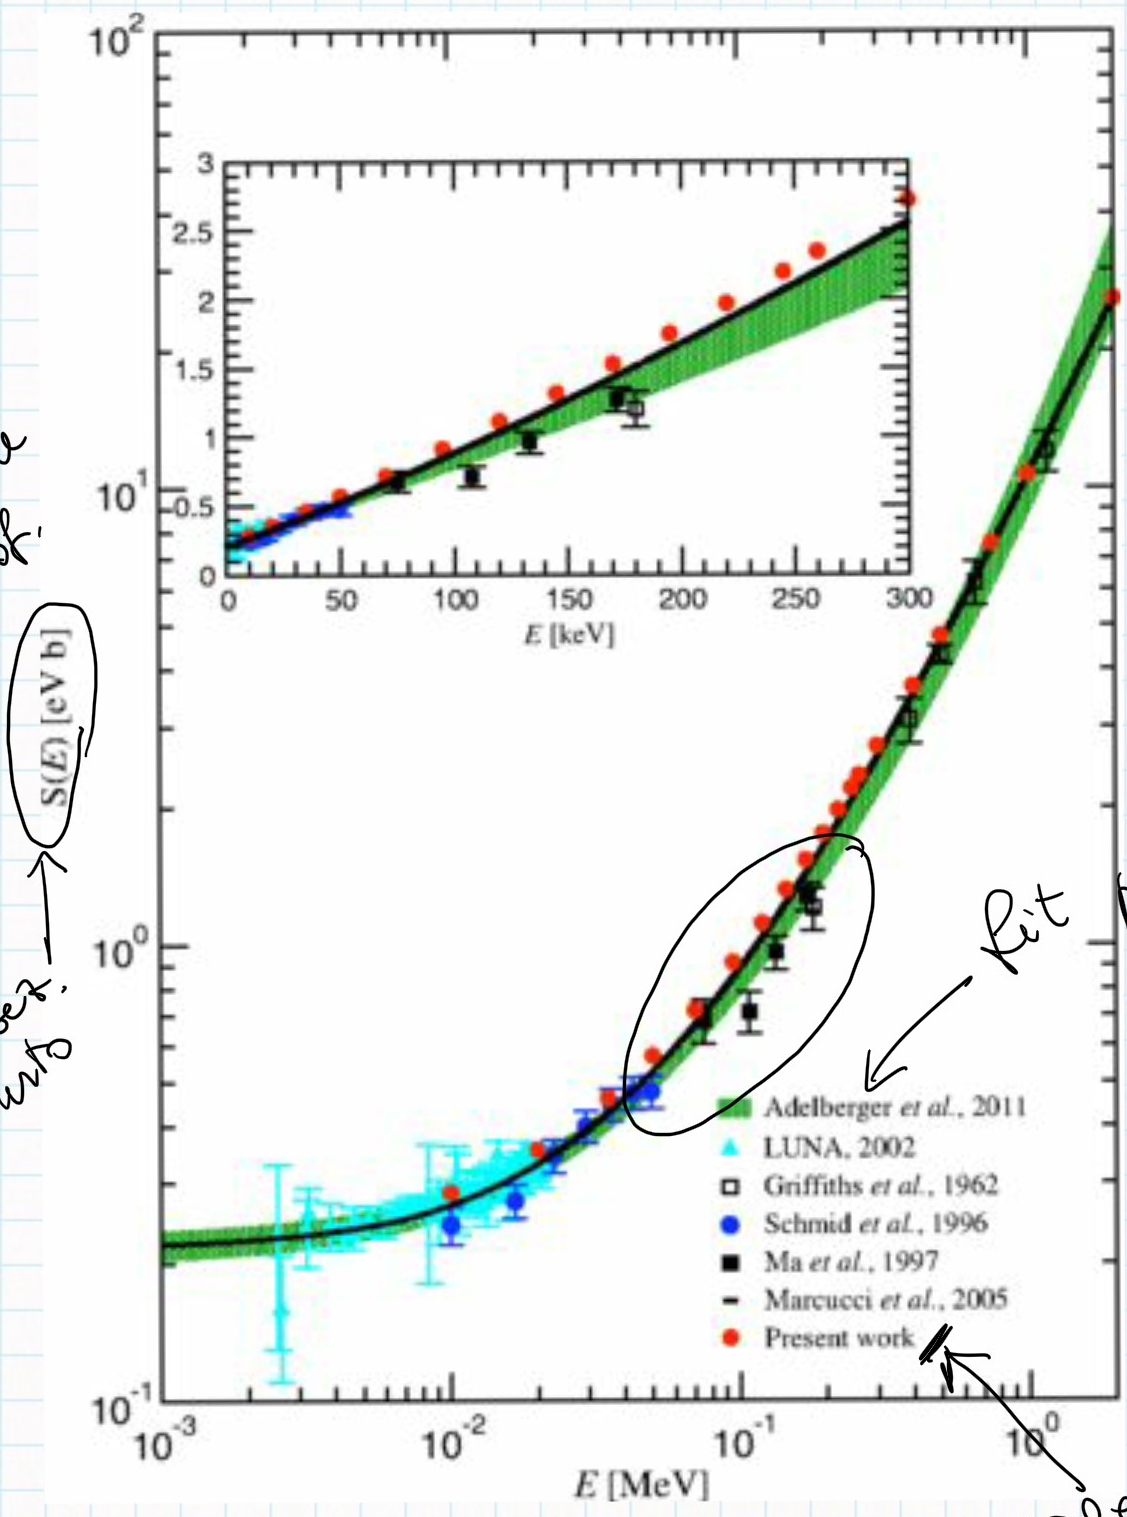
\includegraphics[scale=0.2]{Immagini/0315_fattoreastr.png}
    \caption{La parte cerchiata è il range di interesse per la BBN. La banda verde corrisponde a un fit polinomiale, i punti rossi ad alcuni calcoli teorici e i punti neri ai dati (che rimangono sotto a tutto).}
    \label{0315_astr}
\end{figure}

% \newpage

\noindent Recentemente in Italia si sono fatte altre prese dati grazie all'esperimento LUNA\esperimento{LUNA}\footnote{che discuteremo ampiamente nella sezione \secrif{sec-LUNA}.}, che ha raggiunto un'incertezza del 3\%. Riportiamo i risultati in Figura \ref{0315_astr2}. Rispetto al precedente, il rate di presa dati era molto maggiore e le misure molto più accurate, grazie un codice numerico detto \textit{PArthENoPE}\index{PArthENoPE@\textit{PArthENoPE}}\footnote{Per info: \url{http://parthenope.na.infn.it}.}, che ritorna le funzioni di \textit{likehood} riportate in Figura \ref{0315_parthenope}\footnote{La differenza tra il calcolo delle linee segnate come \textit{Marcucci} è dovuta alle funzioni d'onda di scattering; si osserva che le misure del 2016 sono più accurate, tuttavia non se ne conosce il motivo.}.

\begin{figure}[h]
    \centering
    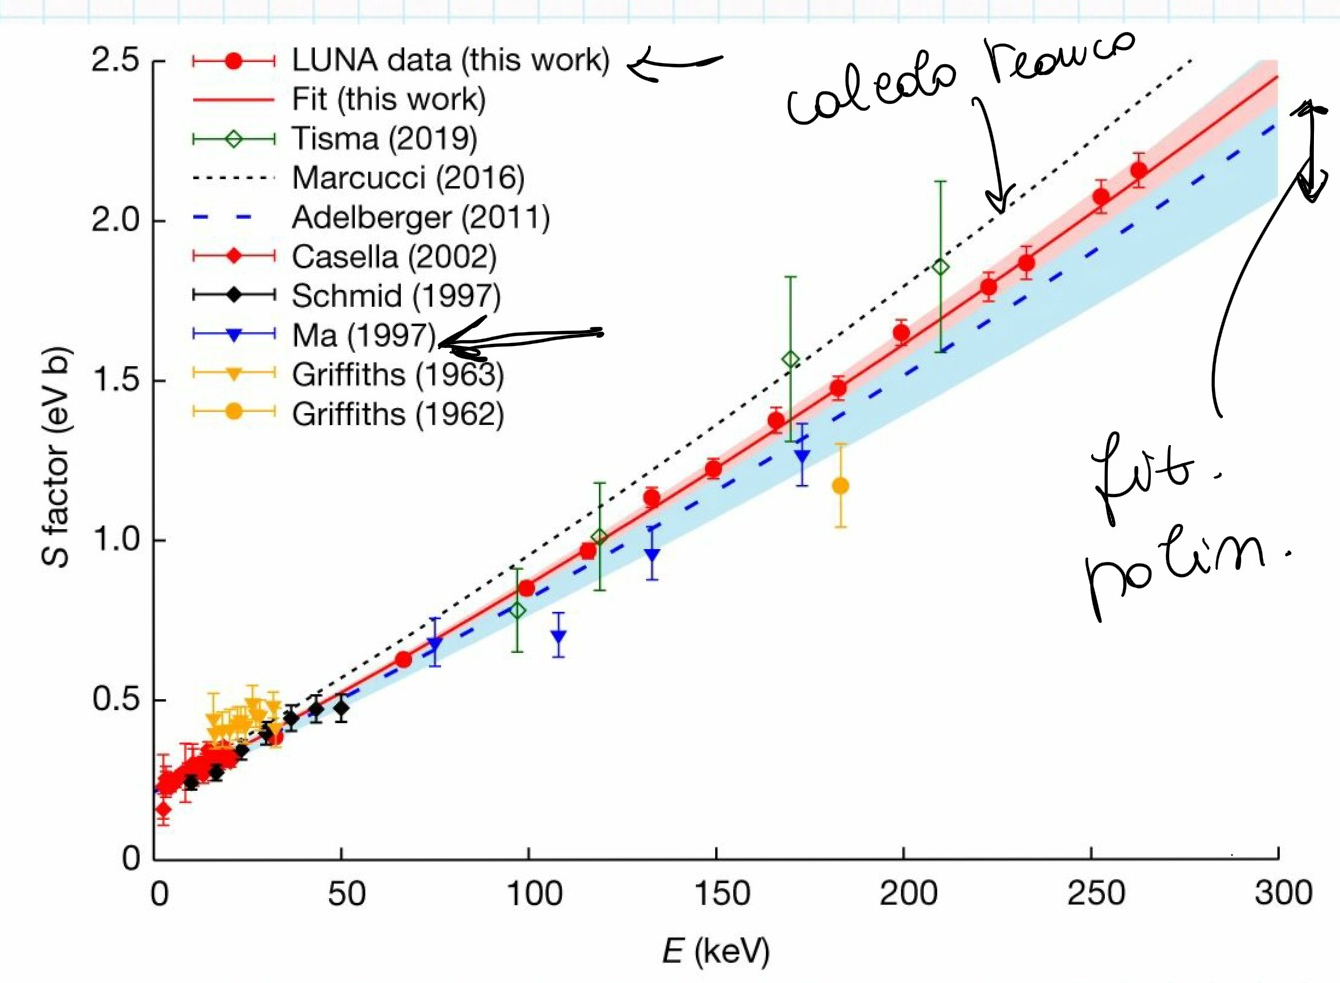
\includegraphics[scale=0.2]{Immagini/0315_fattoreastr2.png}
    \caption{I dati blu sono quelli che nella figura precedente erano segnati in nero. Quelli rossi sono i nuovi dati, la banda celeste corrisponde al fit polinomiale e la linea tratteggiata è l'andamento teorico. I dati di Casella 2002 (basse energie) sono quelli di LUNA I, mentre i dati in rosso circolari sono quelli di LUNA II (vedi \secrif{sec-LUNAII}).}
    \label{0315_astr2}
\end{figure}



\begin{figure}[!h]
    \centering
    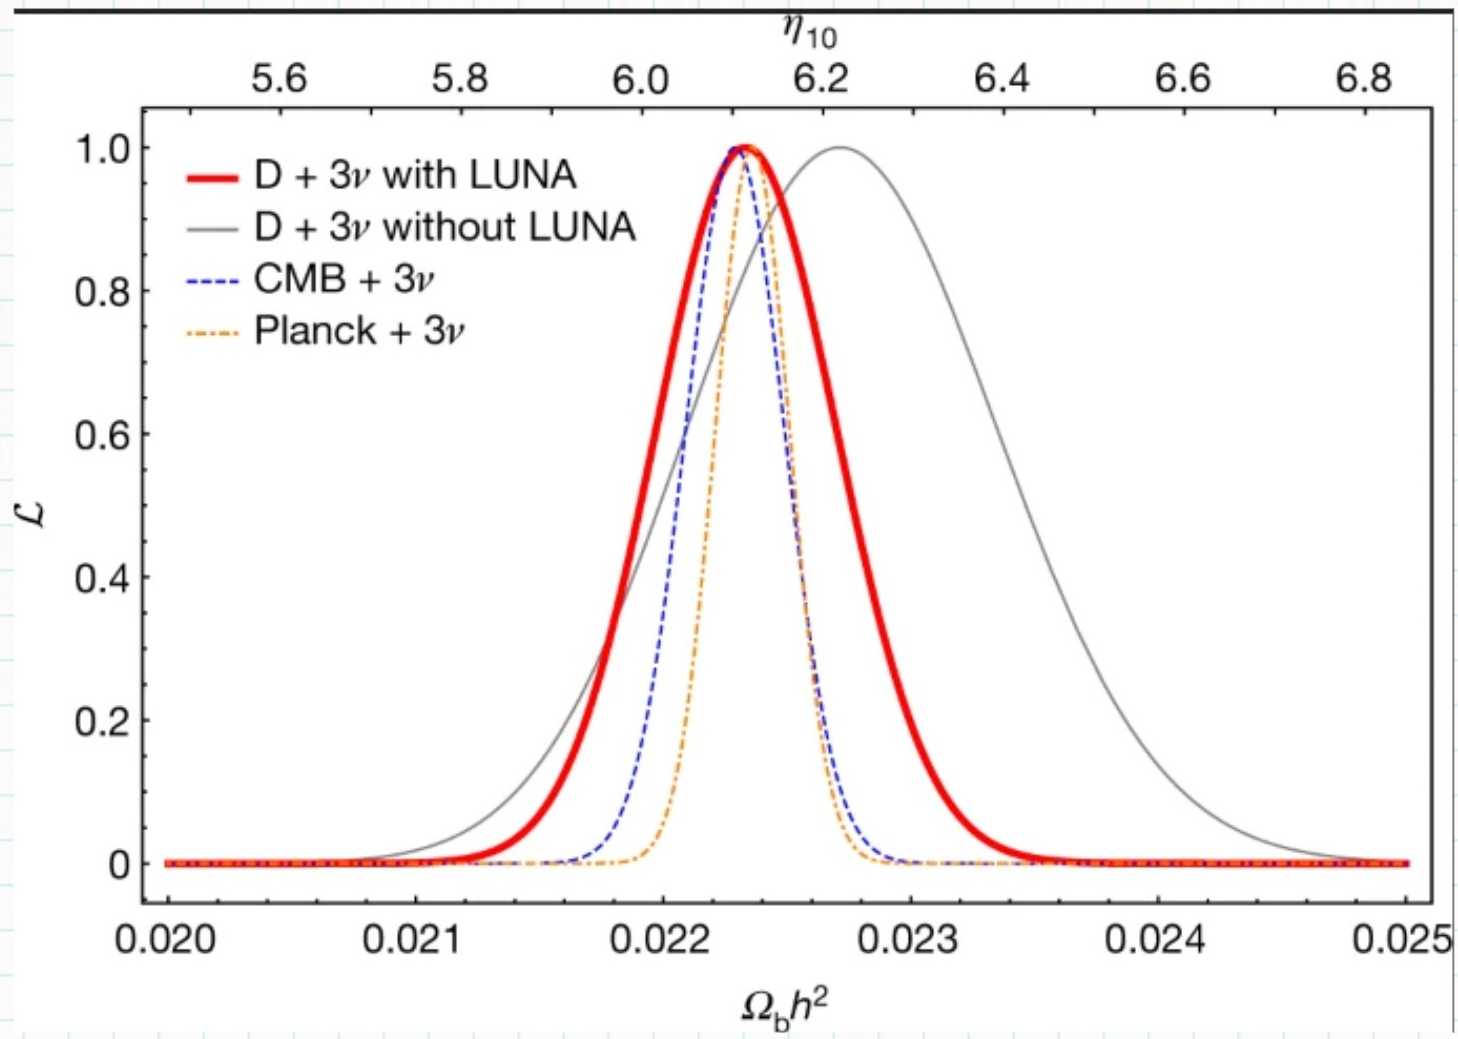
\includegraphics[scale=0.2]{Immagini/0315_luna.png}
    \caption{Risultati per i vari esperimenti ottenuti tramite \textit{PArthENoPE}.}
    \label{0315_parthenope}
\end{figure}
% \newpage
\noindent Dato $\Omega_B h^2$ da Planck, è possibile predire $d/\ce{H}|_\text{BBN} = (2.52\pm0.03\pm0.06)\cdot\ord{-5}$ da confrontare con il valore $\Omega_B$ più probabile ottenuto attraverso l'algoritmo. Riportiamo in Figura \ref{0315_risultati} i risultati di LUNA, che hanno mostrato come non ci sia \textit{nuova fisica} in questo campo: vi è un forte accordo tra il modello standard $\Lambda CDM$ e la teoria della BBN.\\
Rimane ancora in sospeso il $\ce{Li}$-\textit{problem}\index{Li-problem@$\ce{Li}$-\textit{problem}}\index{Li-puzzle@$\ce{Li}$-\textit{puzzle}}, ma le ipotesi più recenti sostengono che probabilmente sia dovuto a un errore nella misurazione dell'abbondanza primordiale del litio.



\begin{figure}[h]
    \centering
    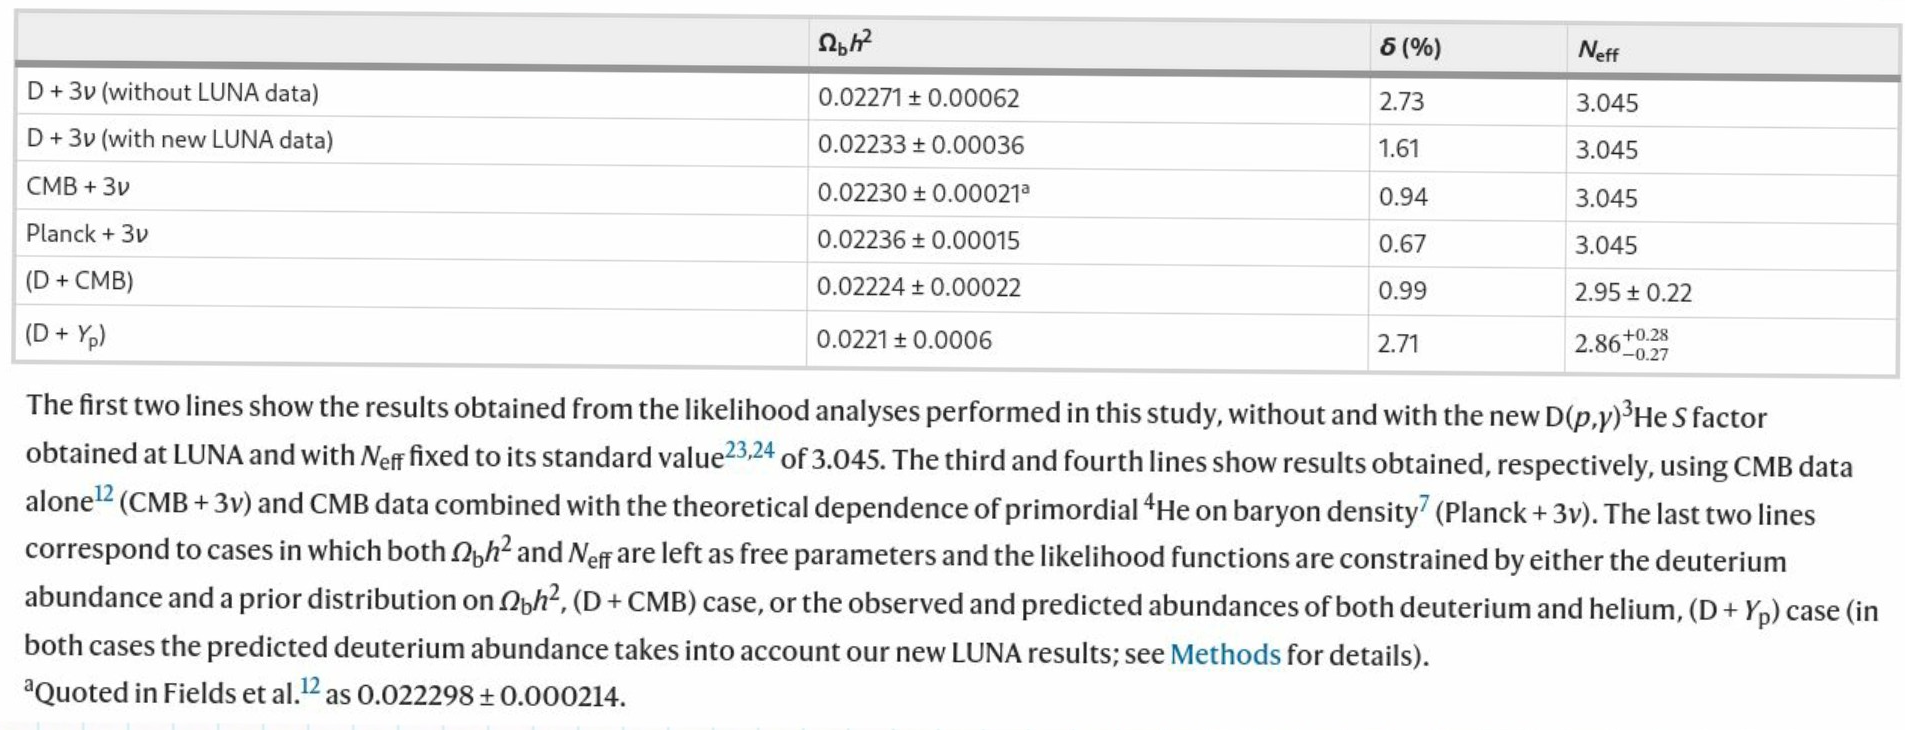
\includegraphics[scale=0.26]{Immagini/0315_risultati.png}
    \caption{Risultati di LUNA. Nei casi delle ultime due righe è stata rilasciato il numero di neutrini, precedentemente fissato dall'abbondanza di elio.}
    \label{0315_risultati}
\end{figure}
\newpage